%Funktionen
%-unit step
%-Impulsfunktion
%-Signumfunktion
%-Rechteckfunktion


\section{Funktionen}
	\subsection{Schrittfunktion - unit step}
		\begin{minipage}{10cm}
			$u(t) = \sigma(t) =	\begin{cases}
						 0 & \text{f\"ur } t < 0 \\
						 \frac{1}{2} \text{(praxis)}  \text{ oder undef. (math.)} & \text{f\"ur } t = 0 \\
						 1 & \text{f\"ur } t > 0
					\end{cases}
			$
			$\sigma(t) \laplace \frac{1}{j\omega} + \pi\delta(\omega) = \Sigma(\omega)$ \\
			$\frac{du(t)}{dt}=\delta(t)$
		\end{minipage}
		\begin{minipage}{8cm}
			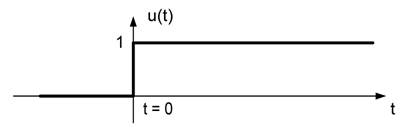
\includegraphics[width=6cm]{./bilder/unitstep.png}
		\end{minipage}

	\subsection{Impulsfunktion - dirac delta function}
		\begin{minipage}{10cm}
			$\delta (t)=\begin{cases} 0 & t\ne 0\\\infty & t=0\end{cases} \qquad
			\text{und} \qquad \int\limits_{-\infty}^\infty \delta(t) \, \mathrm dt = 1 $\\
			$\int\limits_{-\infty}^{\infty}\delta(t-t_0)f(t)dt=f(t_0)$\\
			$\int\limits_{-\infty}^{\infty}\delta(at)\cdot f(t) dt = \frac{1}{|a|} \cdot f(0)$\\
			$s(t) \cdot \delta(t-t_0) = s(t_0)\cdot \delta(t-t_0)$\\
			Fouriertransformierte von $\delta(t)$:\\
			$\delta(t) \laplace 1(\omega)$\\
			$\delta(t-t_0) \laplace e^{-j\omega t_0}$\\
			$1(t) \laplace 2\pi \delta(\omega)$
		\end{minipage}
		\begin{minipage}{8cm}
			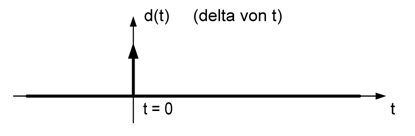
\includegraphics[width=6cm]{./bilder/diracimpulse.png}
		\end{minipage}
		
	\subsection{Signumfunktion}
		\begin{tabular}{p{6cm} p{6cm} p{6cm}}
			$sgn(t) = \begin{cases} 1 & \text{falls }t > 0 \\ -1 & \text{falls }t < 0 \end{cases}$ &
			$sgn(t) \laplace \frac{2}{j\omega}$ &
			$\frac{1}{\pi t} \laplace -j sgn(\omega)$
		\end{tabular}
		
	\subsection{Rechteckimpuls}
		\begin{tabular}{p{9cm} p{9cm}}
			$r_T(t) \laplace \frac{2}{\omega} \cdot \sin(\omega T) \Rightarrow$ sinc-Funktion &
			$\int\limits_{-\infty}^{\infty} \frac{\sin(a \omega)}{\omega} d\omega = 
			\begin{cases} \pi & \text{falls }a > 0 \\ -\pi & \text{falls }a < 0 \end{cases}$
		\end{tabular}